\documentclass{standalone}
\usepackage{tikz}
\begin{document}
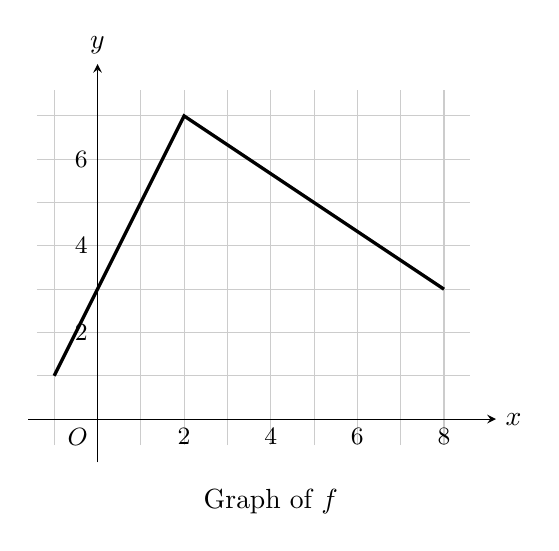
\begin{tikzpicture}[>=stealth, x=0.55cm, y=0.55cm]
  % Graph of f on [-1, 8]: two line segments
  %   (-1, 1) to (2, 7), slope 2 (f(0) = 3, f'(x) = 2 on -1 < x < 2)
  %   (2, 7) to (8, 3), slope -2/3
  \foreach \x in {-1,...,8} { \draw[gray!40] (\x,-0.6) -- (\x,7.6); }
  \foreach \y in {1,...,7} { \draw[gray!40] (-1.4,\y) -- (8.6,\y); }
  \draw[->] (-1.6,0) -- (9.2,0) node[right] {$x$};
  \draw[->] (0,-1) -- (0,8.2) node[above] {$y$};
  \foreach \x in {2,4,6,8} {
    \node[below, font=\small] at (\x,0) {$\x$};
  }
  \foreach \y in {2,4,6} {
    \node[left, font=\small] at (0,\y) {$\y$};
  }
  \node[below left, font=\small] at (0,0) {$O$};
  \draw[very thick] (-1,1) -- (2,7) -- (8,3);
  \node at (4,-1.9) {Graph of $f$};
\end{tikzpicture}
\end{document}
